\chapter{Mengenal Kecerdasan Buatan dan Scikit-Learn}

\begin{enumerate}
\item
Mengerti definisi kecerdasan buatan, sejarah kecerdasan buatan, perkembangan dan penggunaan di perusahaan
\item
Memahami cara instalasi dan pemakaian sci-kit learn
\item
Memahami cara penggunaan variabel explorer di spyder
\end{enumerate}
Tugas dengan cara dikumpulkan dengan pull request ke github dengan menggunakan latex pada repo yang dibuat oleh asisten riset.

\section{Teori}

Kecerdasan Buatan merupakan sebuah rekayasa kecerdasan yang diterapkan ke dalam komputer, diprogram dengan tujuan berfikir dan meniru tindakan manusia \cite{jmcai}. Di dalam kecerdasan buatan terdapat proses pengumpulan informasi, penalaran dan koreksi untuk mencapai hasil yang diharapkan.\cite{jfai}
\\
\\
\subsection{Sejarah}
Pada tahun 1943 hingga 1955 menjadi sebuah cikal bakal kecerdasan buatan lahir. Warren Mc Culloch dan Walter Pitts mengusulkan model neuron buatan yang dimana setiap neuron diindikasikan sebagai “hidup” atau “mati”, dengan sakelar “hidup” terjadilah respon terhadap stimulasi oleh neuron lain. Mereka membuatnya dengan memanfaatkan tiga sumber : \textit{Knowledge of the basic physiology and function of neurons in the brain;} \textit{A formal analysis of propositional logic due to Russell and Whitehead}; dan \textit{Turing’s theory of computation}.
\\
\\
Di tahun 1956, nama Artificial Intelligence pertama tercetus dari John McCarthy. McCarrthy menggaet Minsky, Claude Shannon, dan Nathaniel Rochester untuk membantunya bergabung dengan  peneliti U.S yang tertarik dalam teori automata, jaringan neuron, dan pembelajaran kecerdasan.  Mereka menyelenggarakan lokakarya yang berlangung dua bulan di Dartmouth, dalam proposalnya menyatakan : 
“Kami mengusulkan bahwa studi kecerdasan buatan selama 2 bulan, 10 orang dilakukan keluar selama musim panas 1956 di Dartmouth College di Hanover, New Hampshire. Studi ini dilakukan atas dasar dugaan bahwa setiap aspek belajar atau fitur kecerdasan lainnya pada prinsipnya dapat ditentukan dengan sangat tepat. menjelaskan bahwa mesin dapat dibuat untuk mensimulasikannya. Upaya akan dilakukan untuk menemukan bagaimana membuat mesin menggunakan bahasa, membentuk abstraksi dan konsep, memecahkan jenis masalah sekarang disediakan untuk manusia, dan memperbaiki diri. Kami berpikir bahwa kemajuan yang signifikan dapat dibuat dalam satu atau lebih dari masalah ini jika hati-hati sekelompok ilmuwan terpilih mengerjakannya bersama selama musim panas.”
John McCarty Mengusulkan definisi Kecerdasan Buatan “Merupakan cabang ilmu yang berfokus pada pengembangan komputer untuk dapat bertindak dan berperilaku layaknya manusia”.\cite{russell2009artificial}
\\
\subsection{Perkembangan Kecerdasan Buatan}
Komputer pada awalnya hanya dapat mengelola data, lalu menghasilkan informasi untuk pengambilan keputusan. Seiring perkembangannya saat ini, komputer dapat mengolah pengetahuan sehingga proses pengambilan keputusan menjadi cepat. Bidang ini digunakan dalam pembuktian teorema dan permainan oleh Allen Newell, lalu Arthur Samuel menerapkan kecerdasan buatan pada permainan catur. Seiiring waktu, perkembangan kecerdasan buatan telah menghasilkan bidang turunan antara lain : Sistem pakar; Pengenalan Ucapan, Pengolahan Citra, Robotika, Neural Network, Fuzzy Logic, dsb.\cite{kb13vic}
\\
\subsection{Metode Pembelajaran}
	Supervised learning merupakan metode yang bertujuan untuk memprediksi variabel target berdasarkan model hasil training menggunakan himpunan data berlabel. Biasanya dipergunakan dalam menyelesaikan masalah komputasi yang dikelompokan menjadi :Klasifikasi (proses pengelompokan berdasarkan ciri ciri yang sama);Regresi (prediksi hubungan antara variabel dependen dan variabel lainnya). Sedangkan unsupervised learning merupakan metode yang bertujuan untuk memprediksi variabel data tanpa adanya target data. Metode ini dipergunakan untuk menyelesaikan masalah secara : Klastering (pengelompokan data training ke dalam beberapa klaster berdasarkan kesamaannya).
\subsection{Data}
Dataset merupakan himpunan data yang berasal dari berbagai informasi dan dikelola menjadi informasi  untuk melakukan keputusan. Data ini akan terbagi menjadi dua jenis yakni : Training set(dataset yang kita latih untuk membuat prediksi pada sebuah algoritma) dan Test set (bagian dataset yang akan diuji untuk meninjau akurasi atau melihat performanya.

\section{Instalasi}
Membuka https://scikit-learn.org/stable/tutorial/basic/tutorial.html. Dengan menggunakan bahasa yang mudah dimengerti dan bebas plagiat. 
Dan wajib skrinsut dari komputer sendiri.
\begin{enumerate}
\item
Instalasi library scikit dari anaconda, mencoba kompilasi dan uji coba ambil contoh kode dan lihat variabel explorer\\
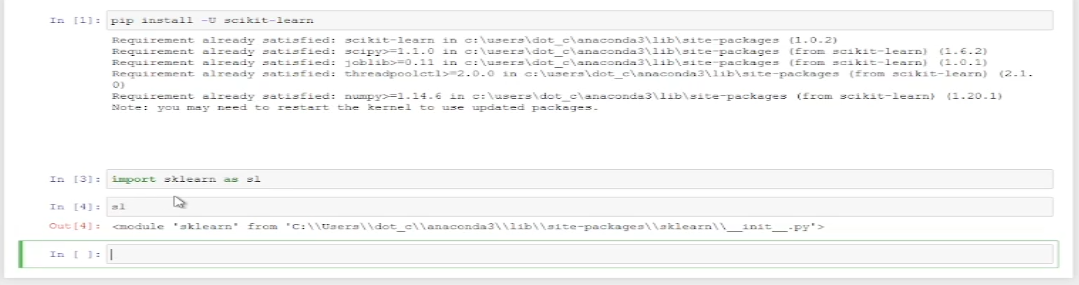
\includegraphics{figures/kb_c1_g1.png}\\
\item
Mencoba Loading an example dataset, menjelaskan maksud dari tulisan tersebut dan mengartikan per baris[hari ke 1](10)
\item
Mencoba Learning and predicting, menjelaskan maksud dari tulisan tersebut dan mengartikan per baris[hari ke 2](10)
\item
mencoba Model persistence, menjelaskan maksud dari tulisan tersebut dan mengartikan per baris[hari ke 2](10)
\item 
Mencoba Conventions, menjelaskan maksud dari tulisan tersebut dan mengartikan per baris[hari ke 2](10)
\end{enumerate}


\section{Penanganan Error}
Dari percobaan yang dilakukan di atas, apabila mendapatkan error maka:

\begin{enumerate}
	\item
	skrinsut error[hari ke 2](10)
	\item
Tuliskan kode eror dan jenis errornya [hari ke 2](10)
	\item
Solusi pemecahan masalah error tersebut[hari ke 2](10)

\end{enumerate}

